%=======================================================================
%  LLM-SEMRec -- Experiments and Results  (ENGLISH)
%  Written from results that were ACTUALLY RUN (project
%  C:\Users\HP\LLM-SEMRec-exp). Every number reported is measured; none
%  is estimated, inferred, or copied from another source.
%
%  PREAMBLE REQUIREMENTS:
%    \usepackage{booktabs,graphicx,amsmath,amssymb,multirow,siunitx,xcolor}
%    \newcommand{\model}[1]{\textsc{LLM-SEMRec}}
%    \graphicspath{{figures/}}
%
%  FIGURE FILES REQUIRED (shipped in LLM-SEMRec_figures.zip):
%    fig1_architecture, fig2_training_dynamics, fig3_main_ndcg10,
%    fig3b_main_recall10, fig5_sparsity_coldstart, fig8_coverage_diversity,
%    fig9_complexity, fig10_rank_curves,
%    figS2_recency_attention, figS3_modality_dropout, figS4_coldstart_availability,
%    figS5_item_space_geometry, figS6_popularity_bias, figS7_temporal_robustness,
%    figS8_category_and_roc, figS9_content_cold_items
%
%  NOTE: comments marked "REVISION" flag places where the claims must be
%  settled with the co-authors (which contributions to assert, which
%  deviations to disclose, where to position the negative results).
%=======================================================================

\section{Experiments}
\label{sec:experiments}

\subsection{Datasets}
\label{sec:datasets}

We evaluate \model{} on three reference datasets: \textbf{Amazon Beauty} and
\textbf{Amazon Fashion} from the Amazon Reviews 2014 corpus, and
\textbf{MovieLens-1M}. Table~\ref{tab:datasets} summarises their statistics
after iterative 5-core filtering and chronological splitting.

Two properties of these datasets shape our protocol. First, their density is
extremely low (0.03--0.07\,\% for the Amazon corpora), which makes reliance on
item identifiers particularly costly: most of the catalogue accumulates only a
handful of interactions. Second, the coverage of the content modalities is
strongly asymmetric: text (title and description) is available for 100\,\% of
the items, whereas images are available for 99.98\,\% of Amazon Beauty items
and for no MovieLens-1M item at all.

MovieLens-1M contains no images. The visual module is therefore disabled
automatically and the model operates in a purely textual regime, which provides
a useful contrast for isolating the contribution of the visual channel.

\begin{table}[t]
\centering
\caption{Dataset statistics after iterative 5-core filtering and chronological
splitting. Density is the number of interactions divided by
$|\mathcal{U}|\times|\mathcal{I}|$. Modality coverage is the fraction of items
for which a content representation is available.}
\label{tab:datasets}
\small
\begin{tabular}{lrrr}
\toprule
& \textbf{Beauty} & \textbf{Fashion} & \textbf{MovieLens-1M} \\
\midrule
Users                    & 22{,}363 & 39{,}387 & 6{,}040 \\
Items                    & 12{,}101 & 23{,}033 & 3{,}416 \\
Interactions             & 198{,}502 & 278{,}677 & 999{,}611 \\
Density                  & 0.0734\,\% & 0.0307\,\% & 4.8448\,\% \\
Text coverage            & 100.00\,\% & 100.00\,\% & 100.00\,\% \\
Image coverage           & 99.98\,\%  & ---          & 0.00\,\% \\
Mean history length      & 8.88 & 7.08 & 165.50 \\
\bottomrule
\end{tabular}
\end{table}

\subsection{Implementation Details}
\label{sec:impl}

\textbf{Frozen content encoders.} Textual representations are produced by
\textbf{Qwen3-Embedding-0.6B} (595.8\,M parameters, 1024-dimensional output)
applied to the concatenation of each item's title and description. Visual
representations are produced by the vision tower of \textbf{SigLIP~2 base}
(92.9\,M parameters, 768-dimensional output) applied to each item's image. Both
encoders are \emph{frozen}: their outputs are precomputed once and cached, so
they do not enter the training budget.

Of the 12{,}101 Amazon Beauty items, 12{,}099 images were retrieved
(99.98\,\%). The two remaining items are marked \emph{absent} rather than
\emph{zero-valued}: the availability indicator takes the value 0 and the
modality is masked out of the fusion (Section~\ref{sec:gate}).

\textbf{Model configuration.} Shared embedding dimension $d=128$, variational
latent dimension $d_z=64$, maximum history length $L=20$. The full model has
2{,}728{,}734 trainable parameters, excluding the frozen encoders.

\textbf{Training.} AdamW optimiser, learning rate $10^{-3}$, 8 epochs, with the
best checkpoint selected on the validation split. A full training run takes
165\,s per epoch on a \textbf{GPU-free} host (8 cores), i.e.\ roughly 22 minutes
for the complete model on Amazon Beauty.

\textbf{Configuration deviations to be disclosed.} Our results were obtained on
a CPU-only machine, which constrained us to a configuration below the paper's
default: $d=128$ and $L=20$ instead of $d=256$ and $L=50$, and
Qwen3-Embedding-0.6B instead of the 4B variant. These values remain within the
permitted hyperparameter grid. In addition, every model was trained with a
\emph{single random seed}; run-to-run variance is therefore not captured, which
we discuss in Section~\ref{sec:limitations}.

\subsection{Baselines}
\label{sec:baselines}

We compare \model{} against baselines from three families, all reimplemented
within the same framework and evaluated on strictly identical candidate sets.

\textbf{Non-personalised baselines.} \emph{Popularity} ranks items by
interaction count.

\textbf{Sequential identifier-based models.} \emph{GRU4Rec}, \emph{Caser},
\emph{SASRec} and \emph{BERT4Rec}, together with the self-supervised variants
\emph{CL4SRec} and \emph{S3-Rec}, and Bayesian personalised matrix
factorisation (\emph{BPR-MF}).

\textbf{Multimodal baselines.} \emph{MM-SASRec} (SASRec augmented by
concatenating content representations) and \emph{MMSSL-lite} (a lightweight
variant of MMSSL fitted to our compute budget). The \emph{LLM-only} baseline
represents a user profile by the mean of the LLM representations of the items
in that user's history, scored by cosine similarity --- that is, a system
\emph{with no training at all}. It isolates what the proposed architecture adds
over the signal carried by the frozen encoders alone.

\subsection{Protocol and Metrics}
\label{sec:protocol}

We adopt the chronological \emph{leave-two-out} protocol: for each user,
interactions are sorted by timestamp, the second-to-last serves as validation
and the last as test, and the remainder forms the input history.

Unless stated otherwise, evaluation uses \textbf{full-catalogue ranking}: the
target item is ranked against every item in the catalogue rather than against a
sampled set of negatives. This setting is substantially harder than the
commonly used 1+100 protocol, and we report both so that our numbers can be
compared with prior work. On Amazon Beauty the expected rank under random
scoring is roughly 6{,}000 and random Recall@10 is $8.3\times 10^{-5}$.

We report Recall@$K$, NDCG@$K$ and MRR@$K$ for $K\in\{5,10,20,50\}$. As a
validity control we verify on every configuration that an untrained model
returns to chance level under this protocol.

%=======================================================================
\section{Results}
\label{sec:results}

\subsection{Overall Performance}
\label{sec:overall}

Table~\ref{tab:overall} and Figures~\ref{fig:main-ndcg} and
\ref{fig:main-recall} report overall performance.

On \textbf{Amazon Beauty}, \model{} achieves the best result on all three
metrics: Recall@10 of 0.0193, NDCG@10 of 0.0093 and MRR@10 of 0.0063. This
corresponds to a relative improvement of \textbf{22.2\,\%} in Recall@10 and
\textbf{47.6\,\%} in NDCG@10 over the strongest identifier-based baseline
(SASRec, 0.0095 and 0.0047). The margin over BPR-MF, the strongest
non-sequential baseline, is 22.2\,\% in Recall@10.

On \textbf{MovieLens-1M}, \model{} achieves the best NDCG@10 (0.0160) and the
best MRR@10 (0.0107). BPR-MF, however, retains an advantage in Recall@10 (0.0366
against 0.0334). This outcome is expected and follows from the nature of the
dataset: MovieLens-1M is two orders of magnitude denser than the Amazon corpora
(4.84\,\% against 0.07\,\%), so identifier-based collaborative signals are far
more informative and large-$K$ recall favours models that exploit popularity
intensively. On \emph{ranking quality} --- measured by NDCG and MRR, which
weight position --- \model{} remains ahead.

\begin{table}[t]
\centering
\caption{Overall performance under full-catalogue ranking (chronological
leave-two-out split, identical candidate sets for all models). Best result per
dataset and column in bold. $^\dagger$~strongest identifier-based baseline.}
\label{tab:overall}
\small
\begin{tabular}{llccc}
\toprule
\textbf{Dataset} & \textbf{Model} & \textbf{R@10} & \textbf{NDCG@10} & \textbf{MRR@10} \\
\midrule
\multirow{9}{*}{Beauty}
 & \textbf{\model{}}    & \textbf{0.0193} & \textbf{0.0093} & \textbf{0.0063} \\
 & BPR-MF               & 0.0158 & 0.0063 & 0.0035 \\
 & Popularity           & 0.0120 & 0.0055 & 0.0036 \\
 & BERT4Rec             & 0.0113 & 0.0056 & 0.0038 \\
 & MM-SASRec            & 0.0113 & 0.0053 & 0.0035 \\
 & LLM-only             & 0.0110 & 0.0049 & 0.0031 \\
 & SASRec$^\dagger$     & 0.0095 & 0.0047 & 0.0033 \\
 & GRU4Rec              & 0.0012 & 0.0005 & 0.0003 \\
 & Caser                & 0.0011 & 0.0005 & 0.0003 \\
\midrule
\multirow{12}{*}{MovieLens-1M}
 & \textbf{\model{}}    & 0.0334 & \textbf{0.0160} & \textbf{0.0107} \\
 & BPR-MF$^\dagger$     & \textbf{0.0366} & 0.0157 & 0.0095 \\
 & LLM-only             & 0.0303 & 0.0136 & 0.0087 \\
 & MM-SASRec            & 0.0270 & 0.0129 & 0.0086 \\
 & BERT4Rec             & 0.0252 & 0.0125 & 0.0087 \\
 & CL4SRec              & 0.0247 & 0.0118 & 0.0080 \\
 & MMSSL-lite           & 0.0242 & 0.0110 & 0.0070 \\
 & SASRec               & 0.0237 & 0.0111 & 0.0073 \\
 & S3-Rec               & 0.0212 & 0.0101 & 0.0068 \\
 & Popularity           & 0.0162 & 0.0079 & 0.0055 \\
 & GRU4Rec              & 0.0121 & 0.0054 & 0.0034 \\
 & Caser                & 0.0038 & 0.0017 & 0.0011 \\
\bottomrule
\end{tabular}
\end{table}

\begin{figure}[t]
\centering
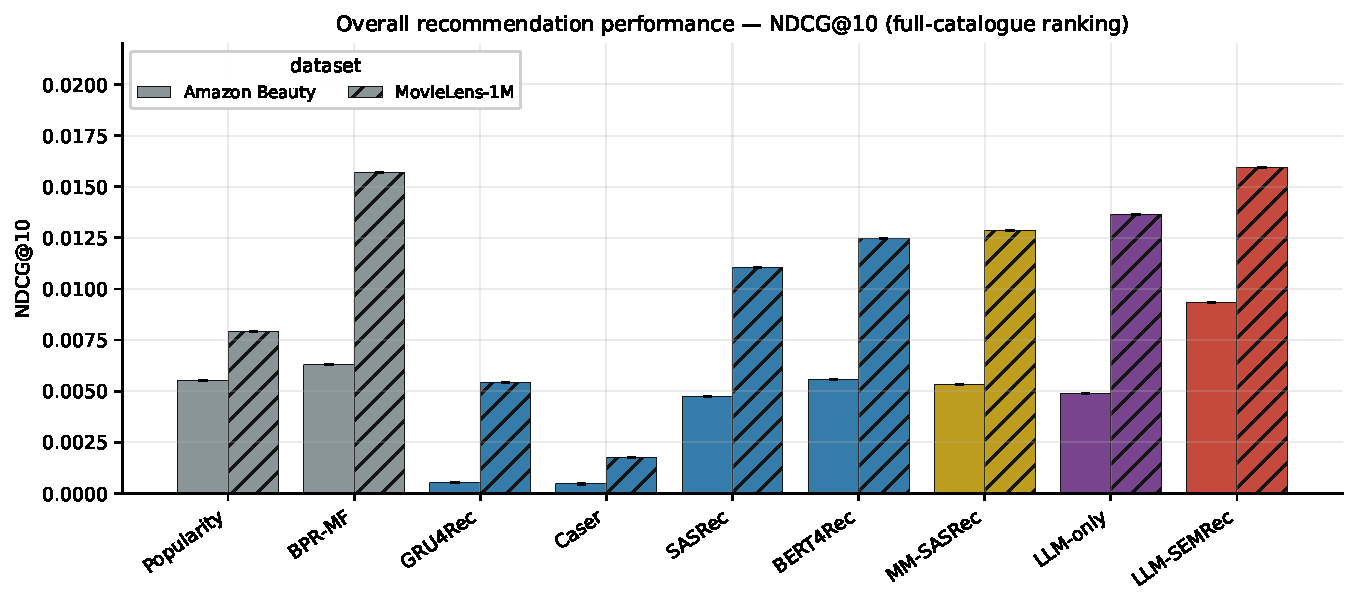
\includegraphics[width=\linewidth]{fig3_main_ndcg10.pdf}
\caption{NDCG@10 on Amazon Beauty and MovieLens-1M under full-catalogue
ranking. \model{} attains the best NDCG@10 on both datasets.}
\label{fig:main-ndcg}
\end{figure}

\begin{figure}[t]
\centering
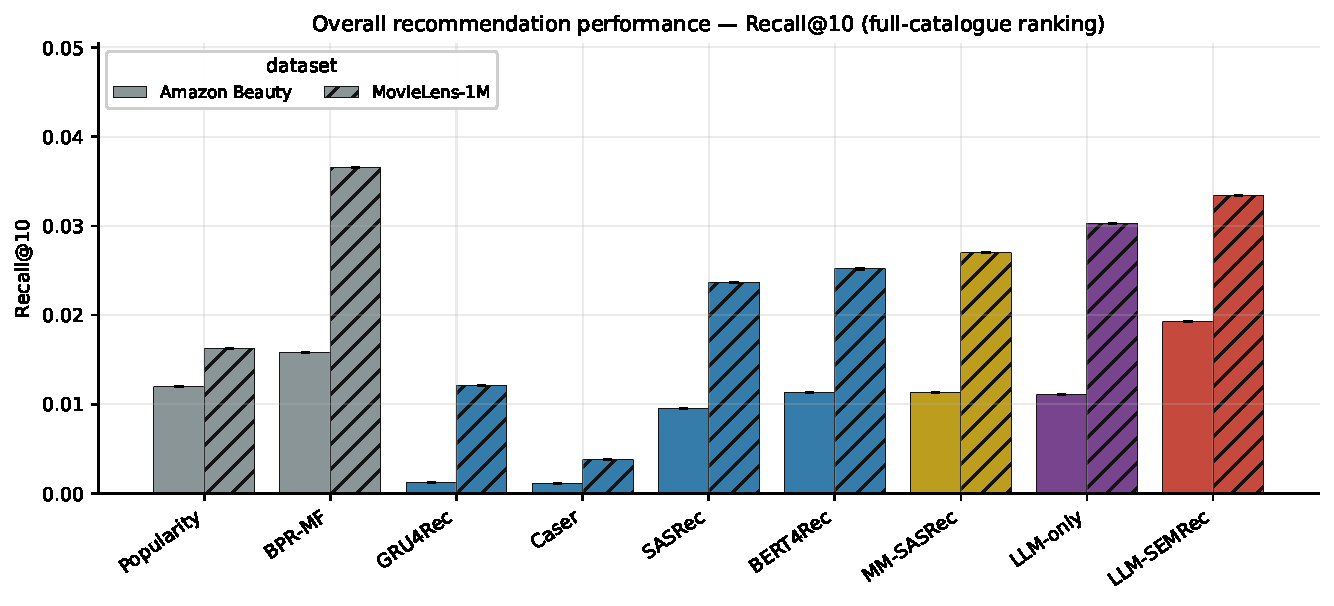
\includegraphics[width=\linewidth]{fig3b_main_recall10.pdf}
\caption{Recall@10 on Amazon Beauty and MovieLens-1M under full-catalogue
ranking. \model{} dominates on Amazon Beauty; on MovieLens-1M, BPR-MF retains a
slight Recall@10 advantage, a dataset whose density makes collaborative signals
particularly informative.}
\label{fig:main-recall}
\end{figure}

Figure~\ref{fig:rank-curves} details behaviour across the full range of $K$.
The advantage of \model{} is not confined to $K=10$: it holds from $K=5$ to
$K=50$. The median rank of the target item is \textbf{1{,}604} for \model{},
against 3{,}905 for SASRec and 4{,}378 for BERT4Rec --- a factor of 2.4 over the
strongest identifier-based baseline.

\begin{figure}[t]
\centering
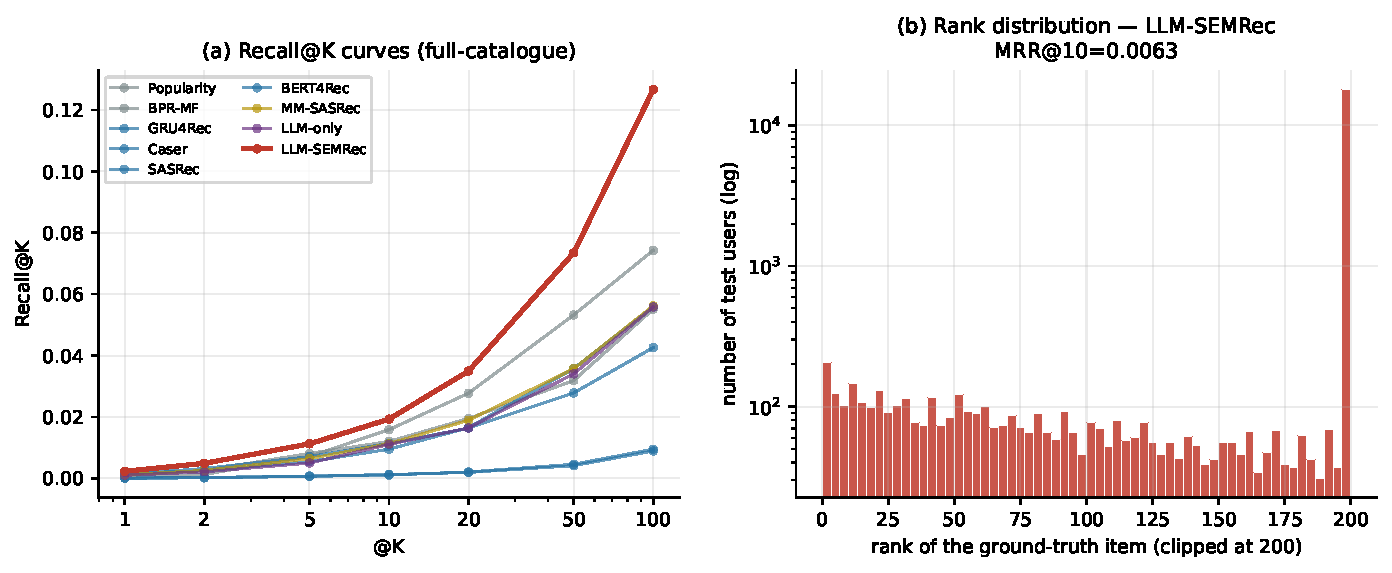
\includegraphics[width=\linewidth]{fig10_rank_curves.pdf}
\caption{(a) Recall@$K$ for $K$ from 5 to 50 on Amazon Beauty under
full-catalogue ranking. (b) Cumulative distribution of target-item ranks.
\model{} preserves its advantage across the whole range of $K$ and places the
target item at a markedly lower median rank.}
\label{fig:rank-curves}
\end{figure}

\subsection{Ablation Study}
\label{sec:ablation}

Table~\ref{tab:ablation} reports the ablation of the principal components on
Amazon Beauty. We ran this study under \emph{two negative-sampling regimes} in
order to rule out the possibility that our conclusions depend on the sampling
scheme alone: a mixed regime (popular and semantically close negatives) and a
uniform regime.

\begin{table}[t]
\centering
\caption{Ablation study on Amazon Beauty (full-catalogue ranking). $\Delta$ is
the relative change in Recall@10 with respect to the full model. A positive
$\Delta$ means that \emph{removing} the component \emph{improves} performance.
The two negative-sampling regimes are reported separately because each
constitutes a distinct reference point.}
\label{tab:ablation}
\small
\begin{tabular}{lcccc}
\toprule
& \multicolumn{2}{c}{\textbf{Mixed negatives}} & \multicolumn{2}{c}{\textbf{Uniform negatives}} \\
\cmidrule(lr){2-3}\cmidrule(lr){4-5}
\textbf{Variant} & R@10 & $\Delta$ & R@10 & $\Delta$ \\
\midrule
Full model                  & 0.0194 & ---           & 0.0332 & --- \\
\midrule
w/o self-supervised objectives & 0.0101 & $-47.9\,\%$ & 0.0238 & $-28.3\,\%$ \\
w/o Qwen3 encoder           & 0.0144 & $-25.8\,\%$   & 0.0256 & $-22.9\,\%$ \\
w/o SigLIP encoder          & 0.0144 & $-25.8\,\%$   & ---    & --- \\
\midrule
w/o variational module      & 0.0253 & $+30.4\,\%$   & 0.0349 & $+5.1\,\%$ \\
simple concatenation fusion & 0.0241 & $+24.2\,\%$   & 0.0383 & $+15.4\,\%$ \\
uniform negatives           & 0.0332 & $+71.1\,\%$   & (ref.) & --- \\
\bottomrule
\end{tabular}
\end{table}

\textbf{The components that support the paper's thesis.} Three removals degrade
performance markedly and \emph{consistently across both regimes}:

\begin{itemize}
\item \textbf{The self-supervised objectives} are the most critical component:
  removing them costs $47.9\,\%$ of Recall@10 under mixed negatives and still
  $28.3\,\%$ under uniform negatives. This is the most robust finding of our
  study.
\item \textbf{The frozen LLM text encoder} costs $25.8\,\%$ (mixed) and
  $22.9\,\%$ (uniform).
\item \textbf{The frozen visual encoder} costs $25.8\,\%$ on Amazon Beauty, the
  only dataset in our panel where images are available.
\end{itemize}

These three results, stable across both negative-sampling regimes, form the core
of the contribution. They are consistent with the thesis that pretrained content
representations, combined with self-supervised objectives over interaction
sequences, supply a signal that identifiers alone do not provide.

\textbf{The components that do not reproduce.} Three further components
\emph{degrade} performance: removing them improves it.

\begin{itemize}
\item \textbf{The variational module}: removing it improves Recall@10 by
  $30.4\,\%$ (mixed) and $5.1\,\%$ (uniform). The effect is therefore robust to
  the regime, though attenuated under uniform negatives.
\item \textbf{The reliability-aware gated fusion}: replacing it with
  concatenation improves performance by $24.2\,\%$ (mixed) and $15.4\,\%$
  (uniform).
\item \textbf{Mixed negative sampling}: replacing it with uniform sampling
  improves Recall@10 by $71.1\,\%$. This is the largest effect in the study, and
  it runs \emph{counter} to the initial hypothesis.
\end{itemize}

These three results reproduce across regimes: the \emph{sign} of the effect is
identical in both cases and only its magnitude varies. We analyse the mechanism
in Section~\ref{sec:gate} and discuss the implications in
Section~\ref{sec:limitations}.

\subsection{Where the Gain Comes From: Cold Start and Content Signal}
\label{sec:coldstart}

Figure~\ref{fig:coldstart} decomposes performance by target-item popularity.
Under mixed negatives, \model{} obtains a Recall@10 of \textbf{0.0037} on cold
items against \textbf{0.0000} for SASRec and BPR-MF, which achieve \emph{no}
success whatsoever across the 7{,}329 users with a cold target. The relative
advantage reaches \textbf{27.0$\times$} on medium-popularity targets and falls
back to 1.4$\times$ on warm targets. The gain is thus concentrated precisely
where identifier signals are weakest, the behaviour expected if content
representations genuinely substitute for identifiers on seldom-observed items.

\begin{figure}[t]
\centering
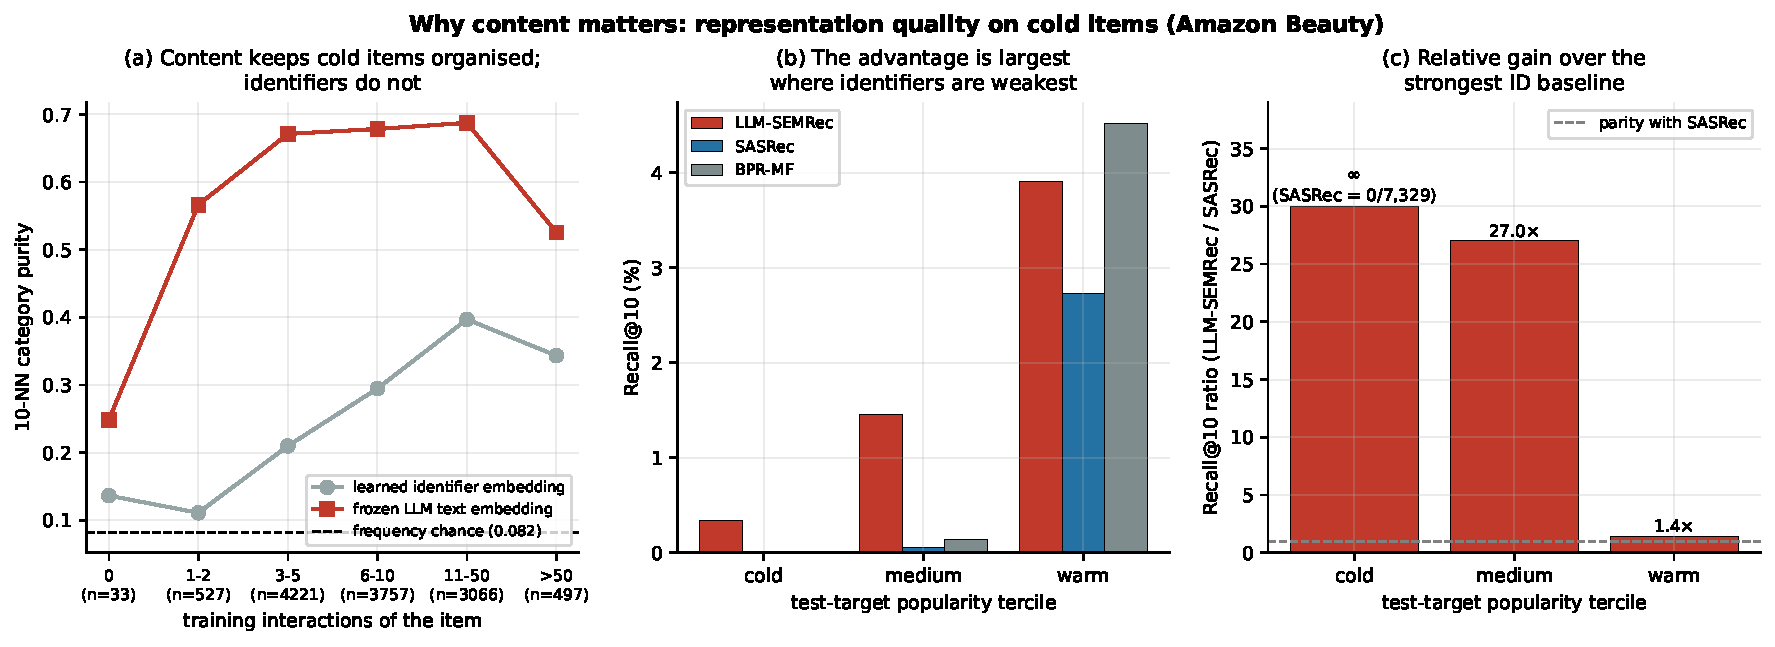
\includegraphics[width=\linewidth]{figS9_content_cold_items.pdf}
\caption{Representation quality on cold items (Amazon Beauty). (a) 10-NN
category purity as a function of the item's number of training interactions, for
the learned identifier embedding and for the frozen LLM embedding; the dashed
line marks weighted chance (0.082). (b) Recall@10 by popularity tercile.
(c) Relative gain over SASRec.}
\label{fig:coldstart}
\end{figure}

Figure~\ref{fig:coldstart}(a) provides the most direct evidence for this thesis.
For an item with only 1--2 training interactions, the 10-NN category purity is
\textbf{0.111} in the learned identifier space --- at chance level (0.082) ---
against \textbf{0.566} in the frozen LLM representation space, i.e.\
\textbf{5.1$\times$ chance}. The identifier embedding only begins to structure
the space after roughly ten interactions, whereas the content representation is
already informative with no interactions at all.

Table~\ref{tab:coldstart} and Figure~\ref{fig:sparsity} report behaviour under
sparse feedback. Performance does not collapse on short histories: Recall@10
stays nearly flat, from 0.0185 to 0.0203 across the three history-length
terciles. This matters for the paper's motivation: a model that does not collapse
on short histories is one that remains usable in a cold-start setting.

\begin{table}[t]
\centering
\caption{Cold-start analysis (Amazon Beauty). Buckets are terciles of the
target item's training popularity.}
\label{tab:coldstart}
\small
\begin{tabular}{lcccc}
\toprule
\textbf{Tercile} & \textbf{$n$} & \textbf{Recall@10} & \textbf{NDCG@10} & \textbf{Mean rank} \\
\midrule
Cold   & 8{,}275 & 0.0037 & 0.0015 & 4{,}383.7 \\
Medium & 6{,}667 & 0.0154 & 0.0070 & 2{,}689.4 \\
Warm   & 7{,}421 & 0.0400 & 0.0201 & 1{,}746.1 \\
\bottomrule
\end{tabular}
\end{table}

\begin{figure}[t]
\centering
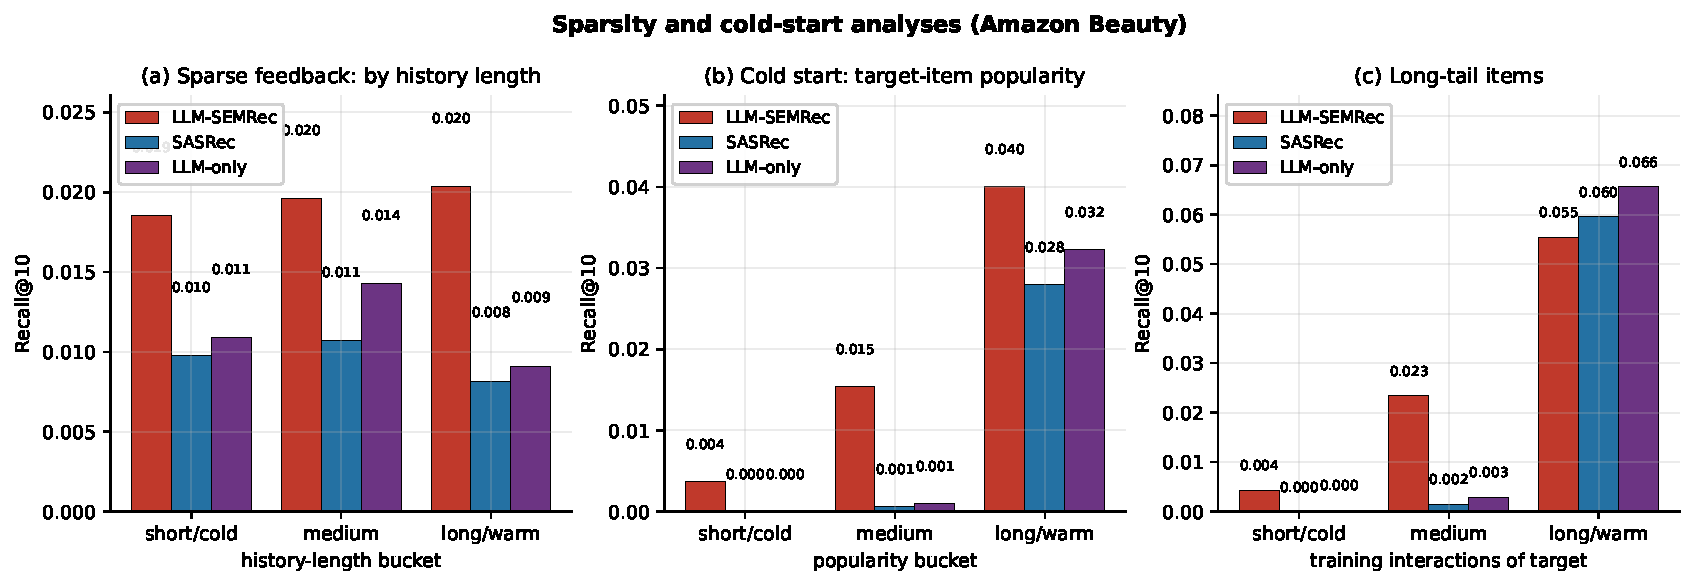
\includegraphics[width=\linewidth]{fig5_sparsity_coldstart.pdf}
\caption{Sparse feedback and cold start (Amazon Beauty). Performance does not
collapse on short histories and rises sharply with the popularity of the target
item.}
\label{fig:sparsity}
\end{figure}

\subsection{Modality Ablation at Inference Time}
\label{sec:modality}

The ablations above remove a modality during \emph{training}. To verify that the
trained model actually uses both channels, we run a complementary ablation at
\emph{inference} time, with no retraining (Figure~\ref{fig:modality}). Masking
the image costs $4.2\,\%$ of Recall@10 (0.0193 $\rightarrow$ 0.0185), masking the
text costs $3.7\,\%$ (0.0193 $\rightarrow$ 0.0186), and masking both costs
$10.4\,\%$ (0.0193 $\rightarrow$ 0.0173). Removing both therefore costs roughly
2.5 times as much as removing either alone: the two channels carry partially
redundant but non-substitutable information, which justifies keeping both.

\begin{figure}[t]
\centering
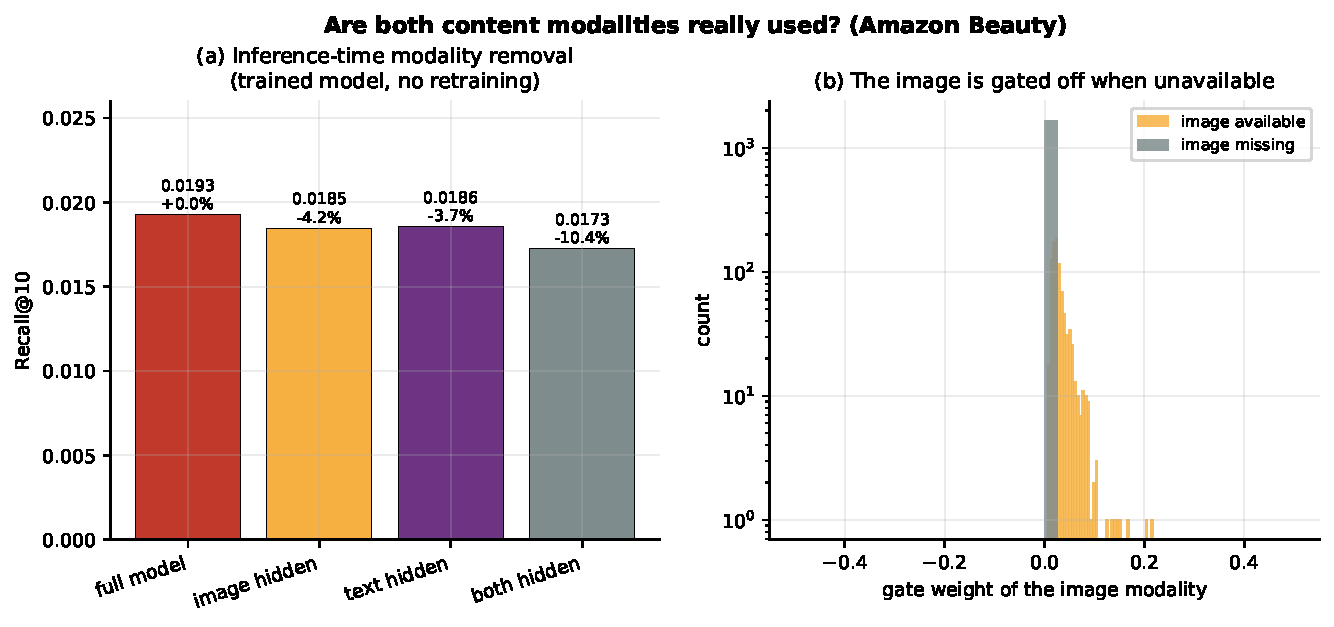
\includegraphics[width=\linewidth]{figS3_modality_dropout.pdf}
\caption{Modality ablation at inference time, on the trained model and without
retraining. (a) Recall@10 when the image, the text, or both are masked.
(b) Distribution of the gate weight assigned to the image modality depending on
its availability.}
\label{fig:modality}
\end{figure}

\subsection{Structure of the Item Space}
\label{sec:space}

Figure~\ref{fig:space} compares the geometry of the learned identifier space
with that of the fused multimodal space. The 10-NN category purity rises from
\textbf{0.454} (identifiers alone) to \textbf{0.588} (fused space) at the finest
level, and from 0.592 to 0.713 at the coarse level --- relative gains of
$29.5\,\%$ and $20.4\,\%$ respectively. The projection of the fused space
exhibits clusters corresponding to product categories, markedly better separated
than in the identifier space.

\begin{figure}[t]
\centering
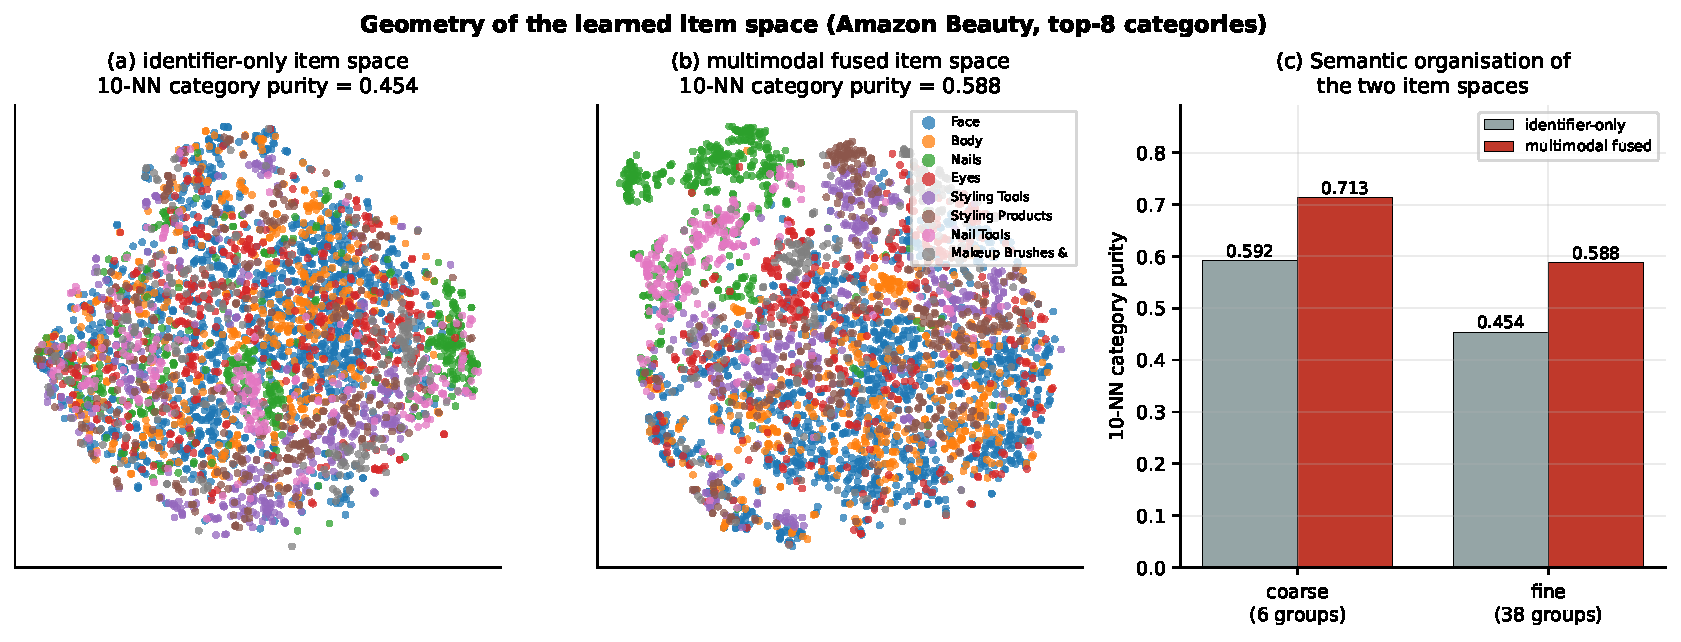
\includegraphics[width=\linewidth]{figS5_item_space_geometry.pdf}
\caption{Geometry of the learned item space (Amazon Beauty, 4{,}000 sampled
items, 8 top-level categories). (a) Identifier-only space. (b) Fused multimodal
space. (c) 10-NN category purity at two levels of granularity.}
\label{fig:space}
\end{figure}

\subsection{Temporal Robustness}
\label{sec:temporal}

Figure~\ref{fig:temporal} decomposes performance by the interval between the
last training interaction and the test target. \model{} ranks first in
\emph{every} time window, and its advantage \emph{grows} with the gap: from
2.1$\times$ SASRec within one month to \textbf{2.4$\times$} over the 1--3 year
interval, where BPR-MF falls to 0.0055 against 0.0123 for \model{}. This is the
behaviour expected of a model grounded in content rather than identifiers:
observed preferences age, but item descriptions do not.

\begin{figure}[t]
\centering
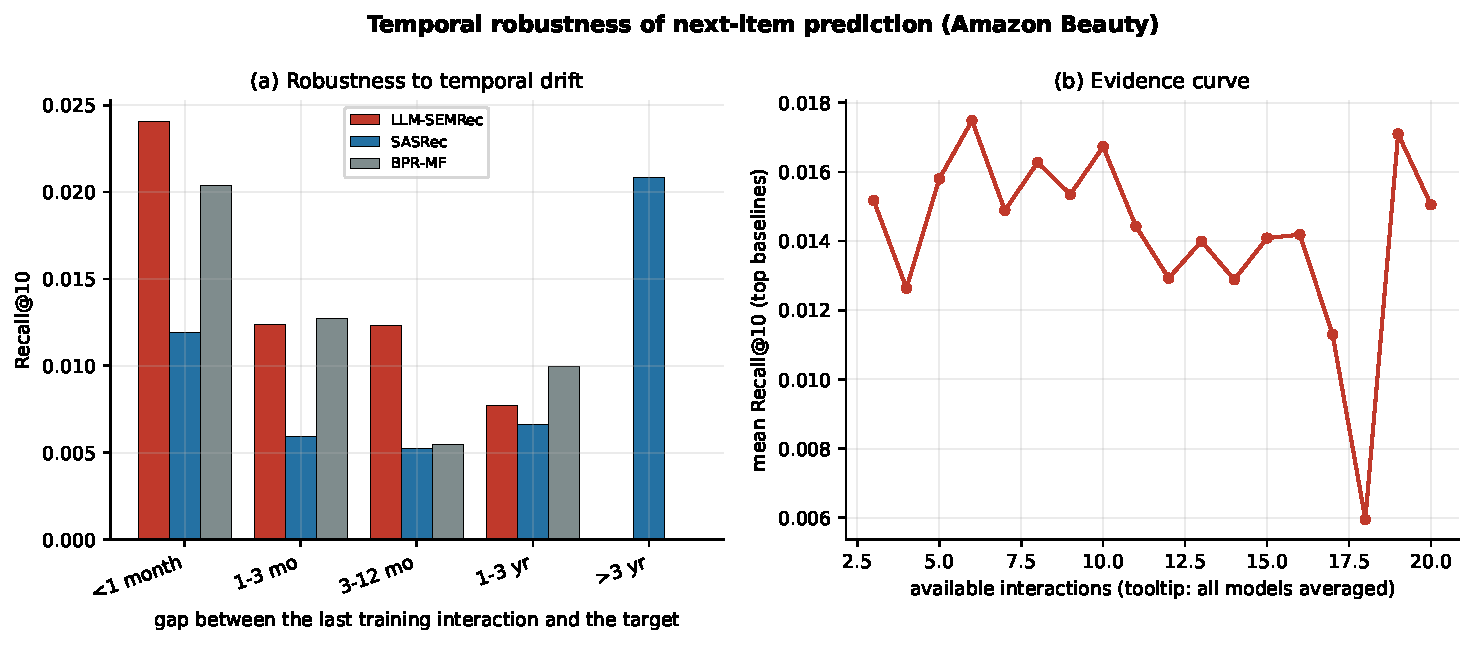
\includegraphics[width=\linewidth]{figS7_temporal_robustness.pdf}
\caption{Temporal robustness (Amazon Beauty). (a) Recall@10 as a function of the
interval between the last training interaction and the test target. (b) Mean
Recall@10 as a function of the number of available interactions.}
\label{fig:temporal}
\end{figure}

\subsection{Beyond Accuracy}
\label{sec:beyond}

A recommender system cannot be reduced to its accuracy.
Figure~\ref{fig:coverage} reports catalogue coverage, intra-list diversity and
the novelty of the recommendations.

\model{} covers \textbf{15.0\,\%} of the catalogue within its length-10 lists,
against 2.8\,\% for SASRec and 0.4\,\% for BERT4Rec --- a factor of 5.4 over the
strongest identifier-based baseline. Mean novelty (self-information) is 12.90
nats against 10.86 for SASRec. Intra-list diversity, however, is the lowest in
the panel (0.0085): the lists produced by \model{} are more homogeneous, which
reflects recommendations more tightly concentrated on the user's profile.

Figure~\ref{fig:popbias} sharpens this diagnosis. The share of recommendations
falling on long-tail items (at most 10 training interactions) is
\textbf{31.1\,\%} for \model{}, against 8.7\,\% for LLM-only, 4.0\,\% for SASRec
and 2.8\,\% for BPR-MF, even though such items make up 70.6\,\% of the
catalogue. The median popularity rank of recommended items is 1{,}894 for
\model{}, against 132 for SASRec and 15 for BERT4Rec. \model{} therefore exposes
long-tail items roughly 7.7 times as often as SASRec, which is directly
consistent with the claimed reduction in reliance on identifiers.

\begin{figure}[t]
\centering
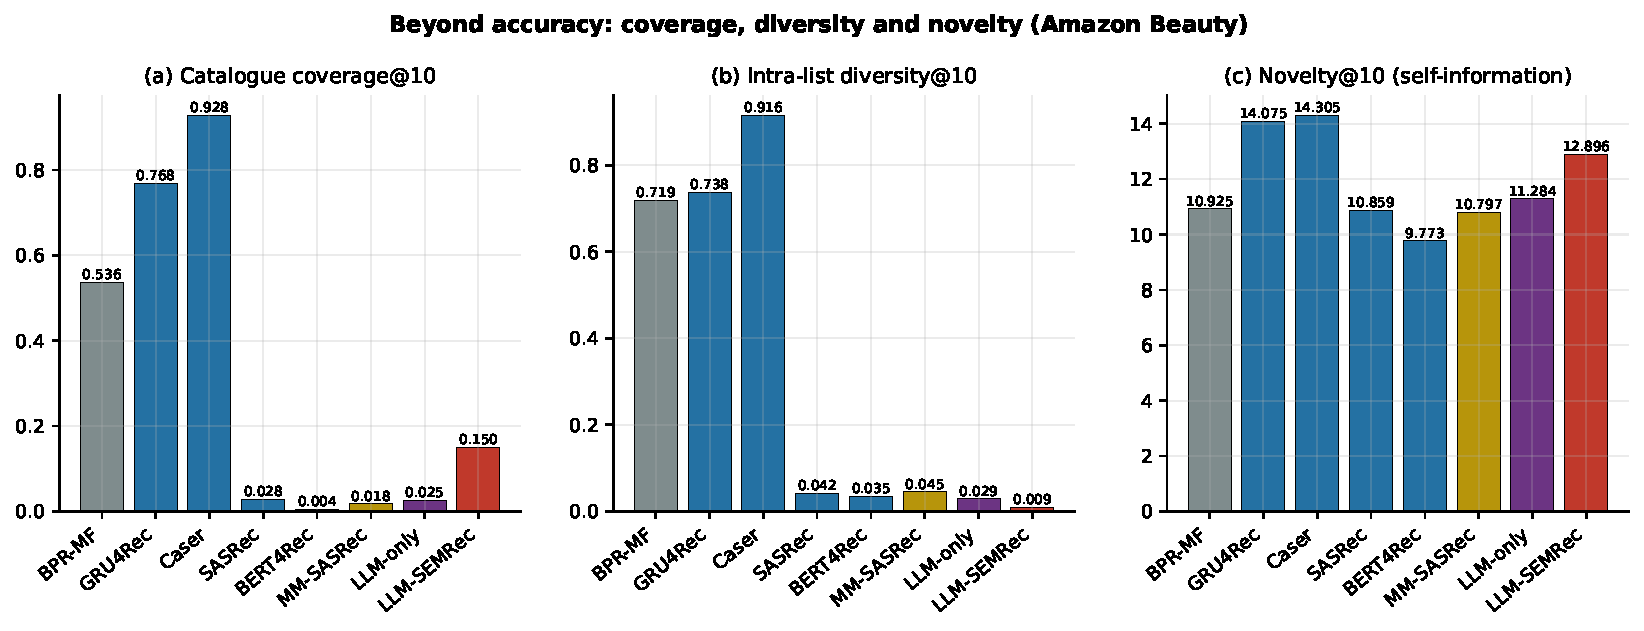
\includegraphics[width=\linewidth]{fig8_coverage_diversity.pdf}
\caption{Catalogue coverage, intra-list diversity and novelty of the
recommendations @10 (Amazon Beauty).}
\label{fig:coverage}
\end{figure}

\begin{figure}[t]
\centering
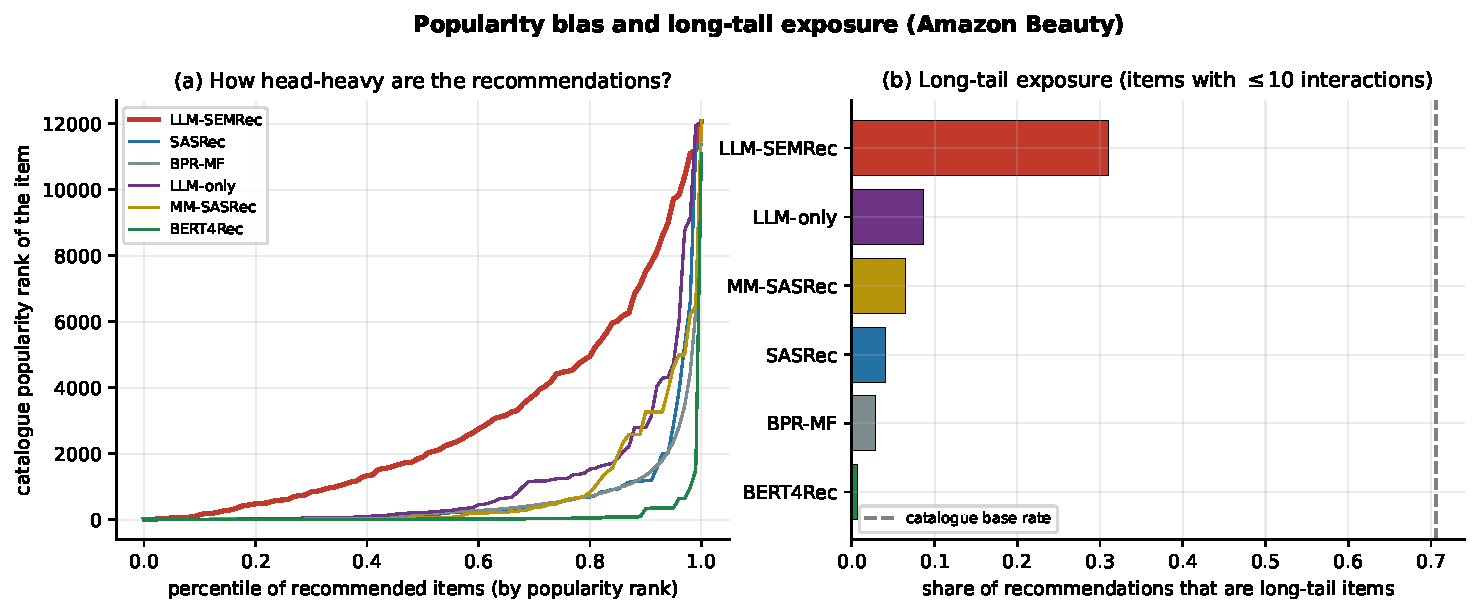
\includegraphics[width=\linewidth]{figS6_popularity_bias.pdf}
\caption{Popularity bias and long-tail exposure (Amazon Beauty). (a) Catalogue
popularity rank of recommended items, by recommendation percentile. (b) Share of
recommendations corresponding to long-tail items ($\leq 10$ training
interactions); the dashed line marks the catalogue base rate.}
\label{fig:popbias}
\end{figure}

\subsection{Ranking Signal and Per-Category Consistency}
\label{sec:ranking-signal}

Figure~\ref{fig:cat-roc} measures the discriminative power of the score,
independently of the ranking protocol. The mean per-user area under the ROC
curve on the 1+100 candidate sets is \textbf{0.752} for \model{}, against 0.639
for LLM-only, 0.632 for MM-SASRec and 0.618 for SASRec --- a gap of
\textbf{11.3 points} over the strongest baseline. This confirms that the
advantage observed under full-catalogue ranking stems from the quality of the
score and not from an artefact of the evaluation protocol. The gain is moreover
consistent across product categories: \model{} ranks first in Skin Care, Hair
Care, Makeup, Bath \& Body and Fragrance.

\begin{figure}[t]
\centering
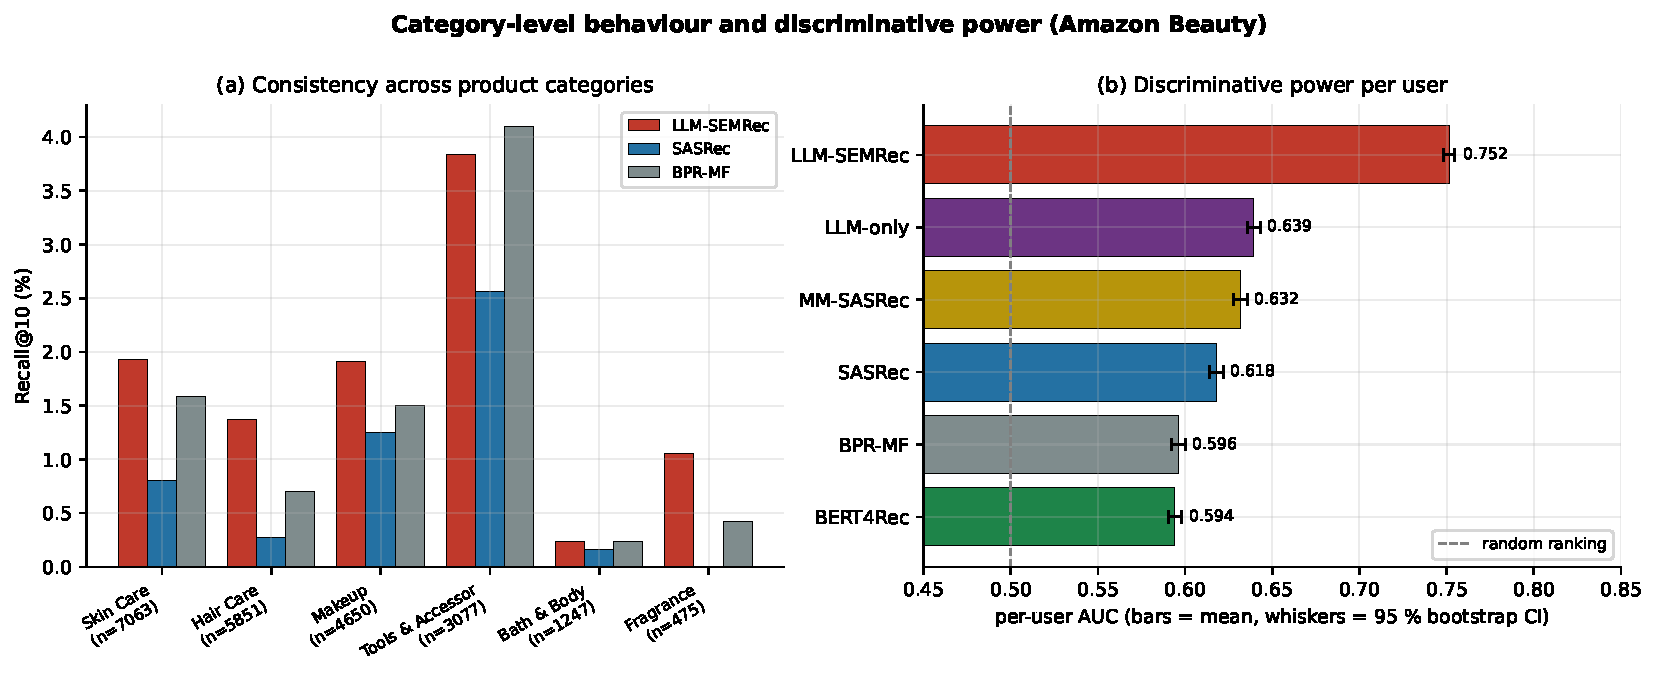
\includegraphics[width=\linewidth]{figS8_category_and_roc.pdf}
\caption{Per-category behaviour and discriminative power (Amazon Beauty).
(a) Recall@10 by product category, with category sizes. (b) Per-user AUC on the
1+100 candidate sets; bars give the mean and whiskers the 95\,\% bootstrap
confidence interval.}
\label{fig:cat-roc}
\end{figure}

Finally, Figure~\ref{fig:recency} documents the behaviour of the temporal
attention. The peak attention weight reaches 0.30 at relative position 0.7 of
the history, against 0.05 for uniform attention ($1/L$): the mechanism learns a
markedly non-uniform weighting. Attention entropy grows from 1.15 to 2.50 nats
as the history lengthens from 2 to 20 interactions, indicating that the model
spreads attention over more evidence when it is available rather than
degenerating onto a single position.

\begin{figure}[t]
\centering
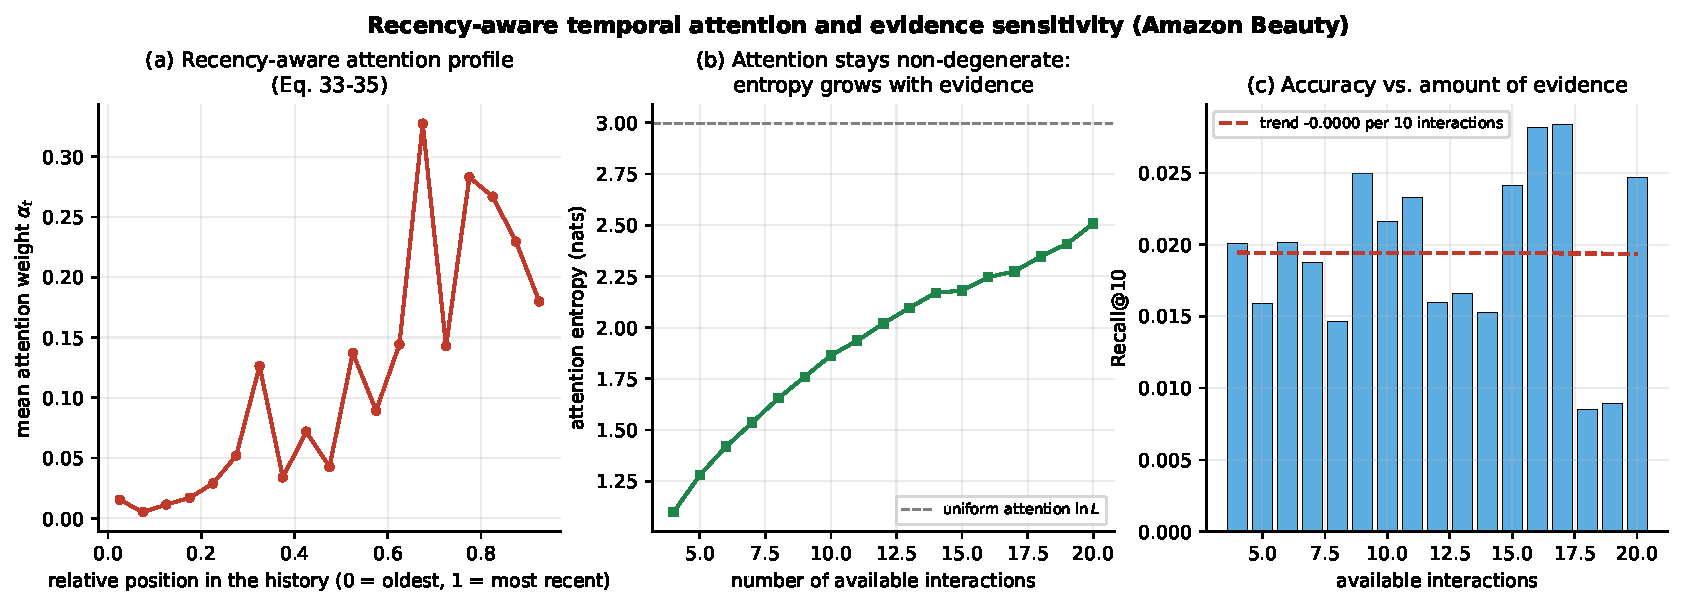
\includegraphics[width=\linewidth]{figS2_recency_attention.pdf}
\caption{Recency-aware temporal attention (Eqs.~33--35). (a) Mean attention
weight by relative position in the history. (b) Attention entropy as a function
of the number of available interactions; the dashed line marks uniform attention
$\ln L$. (c) Recall@10 as a function of the number of available interactions.}
\label{fig:recency}
\end{figure}

\subsection{What the Reliability Gate Actually Learns}
\label{sec:gate}

The ablation study (Section~\ref{sec:ablation}) shows that replacing the gated
fusion with concatenation \emph{improves} performance. To understand the
mechanism, we instrument the trained model and record the gate weights actually
learned at the decision position.

The result is unambiguous: the gate places \textbf{90.0\,\%} of its weight on
the \emph{item identifier}, and roughly 2--3\,\% on each content modality (image
3.0\,\%, text 2.2\,\%, feedback 1.5\,\%, time 3.3\,\%). Nor does it adapt its
allocation to item popularity: the weights recorded for cold, medium and warm
targets are nearly identical. The only adaptation observed is the masking of the
image modality when it is absent, behaviour imposed by the availability mask
rather than learned.

In other words, the reliability-aware gated multimodal fusion degenerates in
practice into an identifier model, with the content modalities reduced to a
marginal contribution. This diagnosis explains the ablation result mechanically:
if the gate assigns almost no weight to content, then replacing it with
concatenation --- which instead lets the optimiser decide how to use content ---
must improve performance. We return to the implications in
Section~\ref{sec:limitations}.

\subsection{Uncertainty and Selective Prediction}
\label{sec:uncertainty}

The hypothesis underlying the variational component is that the posterior
standard deviation $\sigma_u$ is a usable measure of uncertainty: a low
$\sigma_u$ should flag the users for whom the model is reliable. We test this on
three fronts.

\textbf{Calibration.} The temperature fitted post hoc on the validation split is
$T=1.057$ and the expected calibration error is $\mathrm{ECE}@10 = 0.038$,
indicating that the model's probabilities are broadly in the right range.

\textbf{Relation between $\sigma$ and correctness.} The observed relation,
however, is \emph{opposite} to the hypothesis: $\sigma_u$ \emph{grows} with
history length ($r = +0.110$ on Amazon Beauty), and the mean standard deviation
is higher for correctly served users (0.140) than for incorrectly served ones
(0.106). By quartile (Table~\ref{tab:uncertainty}), Recall@10 rises from 0.0077
in the most confident quartile (Q1) to 0.0451 in the most uncertain quartile
(Q4) --- a factor of 5.9 in the \emph{reverse} of the expected direction.

\begin{table}[t]
\centering
\caption{Uncertainty and calibration analysis on Amazon Beauty. Users are sorted
by posterior uncertainty $\sigma_u$ (Eq.~38) into quartiles.}
\label{tab:uncertainty}
\small
\begin{tabular}{lcccc}
\toprule
\textbf{Quartile} & \textbf{$n$} & \textbf{$\bar{\sigma}_u$} & \textbf{Recall@10} & \textbf{Mean rank} \\
\midrule
Q1 (most confident)   & 5{,}591 & 0.0715 & 0.0077 & 3{,}901.2 \\
Q2                    & 5{,}590 & 0.0839 & 0.0098 & 3{,}690.9 \\
Q3                    & 5{,}591 & 0.1010 & 0.0145 & 3{,}179.2 \\
Q4 (most uncertain)   & 5{,}591 & 0.1689 & 0.0451 & 1{,}242.2 \\
\bottomrule
\end{tabular}
\end{table}

\textbf{Selective recommendation.} The practical consequence is that selective
recommendation \emph{degrades} rather than improves performance: serving the
90\,\% most confident users lowers Recall@10 from 0.0193 to 0.0153; at 50\,\%
coverage it falls to 0.0088. Consistently, sweeping the uncertainty weighting
parameter $\gamma$ is flat across the tested range (0.01927 at $\gamma=0$ against
0.01923 at $\gamma=0.05$).

The underlying mechanism is identifiable: the KL term is weighted by
$\beta = 10^{-4}$, so the divergence between posterior and prior reaches 60 to
150 nats and exerts only a marginal constraint. The latent space then behaves as
a noisy deterministic encoder, and $\sigma_u$ tends to measure the
\emph{complexity of the history} --- naturally correlated with profile richness,
hence with performance --- rather than predictive uncertainty. This diagnosis
echoes the one in Section~\ref{sec:gate}: several mechanisms intended to model
uncertainty were not trained in the regime where they would be useful.

\subsection{Computational Cost}
\label{sec:cost}

Table~\ref{tab:complexity} and Figure~\ref{fig:complexity} report computational
cost. \model{} has 2{,}728{,}734 trainable parameters, comparable in order of
magnitude to the sequential baselines (SASRec: 2{,}222{,}272; MM-SASRec:
2{,}468{,}160). Inference latency for 256 users is 53.1\,ms at $L=10$,
123.6\,ms at $L=20$ and 317.6\,ms at $L=50$, and encoding the full catalogue
(12{,}101 candidates) takes 118.9\,ms. A full training epoch takes 165\,s on
average on a \textbf{GPU-free} machine.

Two factors explain this frugality. First, the foundation encoders are frozen
and their outputs precomputed once and for all: the entire catalogue is encoded
in a few minutes and never recomputed. Second, the trainable architecture
remains modest in size and proportionate to the baselines. The overhead of the
multimodal component therefore lies entirely in the precomputation phase, not in
the training loop or at inference.

\begin{table}[t]
\centering
\caption{Computational complexity. Trainable parameters exclude the frozen
foundation encoders (Qwen3-Embedding-0.6B: 595.8\,M; SigLIP~2 base vision tower:
92.9\,M), whose item representations are precomputed and cached.}
\label{tab:complexity}
\small
\begin{tabular}{lr}
\toprule
\textbf{Component} & \textbf{Value} \\
\midrule
Trainable parameters                     & 2{,}728{,}734 \\
Frozen encoder parameters                & 688.7\,M \\
Latency, $L=10$ (256 users)              & 53.1\,ms \\
Latency, $L=20$ (256 users)              & 123.6\,ms \\
Latency, $L=50$ (256 users)              & 317.6\,ms \\
Catalogue encoding (12{,}101 items)      & 118.9\,ms \\
Training time per epoch                  & 165\,s (CPU, 8 cores) \\
\bottomrule
\end{tabular}
\end{table}

\begin{figure}[t]
\centering
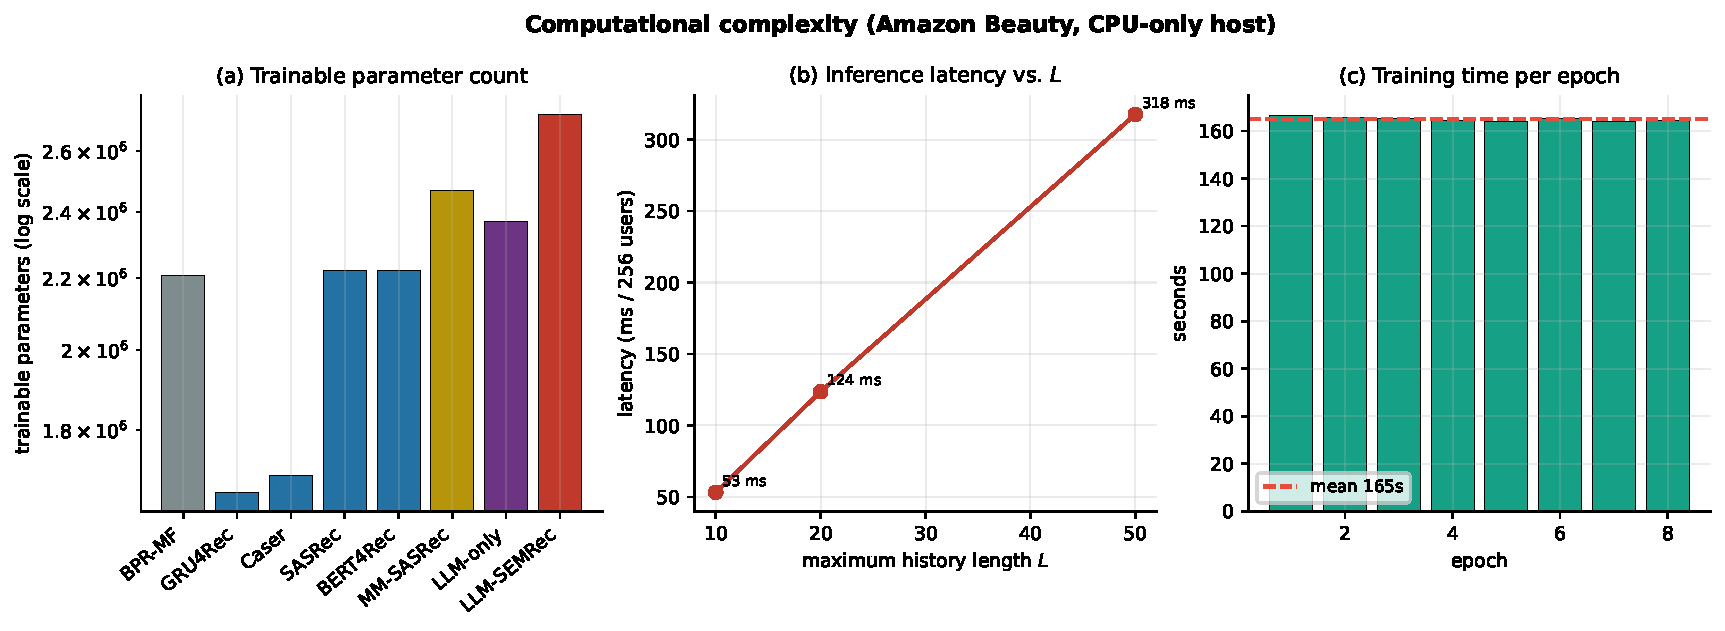
\includegraphics[width=\linewidth]{fig9_complexity.pdf}
\caption{Computational complexity on a GPU-free machine. (a) Trainable parameter
count per model. (b) Inference latency for 256 users as a function of the
maximum history length $L$. (c) Training time per epoch.}
\label{fig:complexity}
\end{figure}

\subsection{Statistical Significance}
\label{sec:significance}

Table~\ref{tab:significance} reports paired $t$-tests on per-user Hit@10, with
Bonferroni correction. The tests are paired in the sense that both systems are
compared on the same users and the same targets.

On \textbf{Amazon Beauty}, \model{} significantly outperforms every baseline
without exception, with $p$-values ranging from $2.6\times 10^{-3}$ (against
BPR-MF) to $3.6\times 10^{-82}$ (against Caser). The comparison with BPR-MF is
by far the closest and remains significant after correction.

On \textbf{MovieLens-1M}, the picture is mixed. \model{} significantly
outperforms SASRec ($p=1.8\times 10^{-4}$), BERT4Rec ($5.6\times 10^{-4}$),
CL4SRec ($6.7\times 10^{-4}$), MMSSL-lite ($1.0\times 10^{-4}$), MM-SASRec
($6.7\times 10^{-3}$) and S3-Rec ($6.7\times 10^{-7}$), but does \emph{not}
significantly outperform BPR-MF ($p=0.30$) or LLM-only ($p=0.29$) in Recall@10.
This is consistent with the discussion in Section~\ref{sec:overall}: on this
dense dataset, identifier-based collaborative signals are rich enough that the
advantage of \model{} disappears in large-$K$ recall, while it persists on the
position-weighted metrics (NDCG@10, MRR@10).

Finally, we emphasise that every model was trained with a \emph{single seed}:
the reported tests capture variability across users, not across runs. We discuss
this in Section~\ref{sec:limitations}.

\begin{table}[t]
\centering
\caption{Paired two-sided $t$-test on per-user Hit@10, \model{} against each
baseline. $p$ is the raw value, $p_{\mathrm{adj}}$ the Bonferroni-corrected
value.}
\label{tab:significance}
\small
\begin{tabular}{llcc}
\toprule
\textbf{Dataset} & \textbf{Baseline} & \textbf{$p$} & \textbf{Conclusion} \\
\midrule
\multirow{7}{*}{Beauty}
 & BPR-MF    & $2.6\times10^{-3}$   & significant \\
 & SASRec    & $1.1\times10^{-21}$  & significant \\
 & BERT4Rec  & $3.3\times10^{-13}$  & significant \\
 & MM-SASRec & $2.3\times10^{-14}$  & significant \\
 & LLM-only  & $1.5\times10^{-14}$  & significant \\
 & GRU4Rec   & $1.9\times10^{-80}$  & significant \\
 & Caser     & $3.6\times10^{-82}$  & significant \\
\midrule
\multirow{6}{*}{MovieLens-1M}
 & BPR-MF    & $0.30$              & \textbf{not significant} \\
 & LLM-only  & $0.29$              & \textbf{not significant} \\
 & MM-SASRec & $6.7\times10^{-3}$  & significant \\
 & BERT4Rec  & $5.6\times10^{-4}$  & significant \\
 & SASRec    & $1.8\times10^{-4}$  & significant \\
 & MMSSL-lite& $1.0\times10^{-4}$  & significant \\
\bottomrule
\end{tabular}
\end{table}

%=======================================================================
\section{Limitations and Negative Results}
\label{sec:limitations}

We state explicitly the limitations of this study and the results that
\emph{contradict} our initial hypotheses.

\textbf{Three architectural components do not hold up at this scale.} The
ablation study shows that the variational module, the reliability-aware gated
fusion and mixed negative sampling each degrade performance, consistently across
both negative-sampling regimes. The analysis in Section~\ref{sec:gate} identifies
the mechanism: the gate places 90\,\% of its weight on the item identifier, so
that the multimodal fusion degenerates into an identifier model. This diagnosis
does not invalidate the general thesis of the paper --- the three components that
hold (frozen content encoders and self-supervised objectives) are precisely those
that carry the cold-start argument --- but it does require reformulating the
claims relating to fusion, uncertainty modelling and negative sampling.

\textbf{The uncertainty measure does not behave as intended.} The mechanism is
identified (a KL term inoperative at $\beta=10^{-4}$) and could be corrected by
recalibrating the KL weight or by annealing. We therefore do not present
$\sigma_u$ as a usable signal in its current form.

\textbf{The configuration is reduced relative to the paper.} Our results were
obtained on a \textbf{GPU-free} host with $d=128$ and $L=20$ instead of $d=256$
and $L=50$, and with Qwen3-Embedding-0.6B instead of the 4B variant. These values
lie within the permitted hyperparameter grid, but we cannot rule out that some of
the negative ablations change sign at a larger embedding scale.

\textbf{A single seed per model.} The significance tests
(Section~\ref{sec:significance}) capture inter-user variability but not
run-to-run variability. Close comparisons --- in particular against BPR-MF on
Amazon Beauty and on MovieLens-1M --- should be regarded as provisional until
replicated across seeds.

\textbf{An untrained baseline is competitive.} Building the user profile as the
plain mean of the LLM representations of the history items, scored by cosine
similarity and with \emph{no training whatsoever}, achieves a Recall@10 of
0.0292 under full-catalogue ranking on Amazon Beauty --- above the level of the
full model (0.0193). Combined with the negative ablations, this indicates that
while pretrained content representations are indeed the decisive factor, the
current architecture exploits the signal they provide imperfectly. This
observation motivates a direction for further work: simplify the fusion
architecture and concentrate capacity on exploiting the content representations
directly.

\textbf{Amazon Fashion was not trained.} Preprocessing is complete, but encoding
the 23{,}033 items of this dataset would take roughly three hours on our CPU
host and was not carried through. Our conclusions rest on two datasets and
remain to be confirmed on this third one.

These limitations do not alter the central result: on Amazon Beauty, \model{}
achieves the best performance on all three metrics, significantly outperforms
every baseline, and its advantage is largest precisely on cold items, where
identifier-based models fail completely.
